% Part 2, Chapter 2: the horizon coefficient eta. Carries the Bekenstein-coefficient paper (Apr 2026; 596 PDF lines, read in full 2026-10-02)
% in its own order, every derivation step, with Jacobson's derivation written out in full (SI units, kappa as an acceleration).
% Corrections applied: PAPER_ERRATA B4 (G = c^3/(4 hbar eta); Eq. 16 factor c; Planck kappa is the maximum; eta still takes G as input),
% B5/N1 (no private correspondent), BLACK_HOLES_CHECK #6 (S propto A argument is interpretation), #11 (Sec. 6.4 not carried).
% Book rules: one nat per 4 l_P^2, one bit per 4 ln2 l_P^2, delta A_min = 4 l_P^2 for any kappa.
% Checks: docs/verification/scripts/verify_bekenstein_bh.py (+ _output.txt), sections B-F and N.

\chapter{The horizon coefficient: why $\eta=1/(4\lP^2)$}\label{ch:bekenstein}

\section*{Overview}
Jacobson's 1995 derivation of the Einstein field equations from thermodynamics~\cite{Jacobson1995} makes two assumptions: entropy proportional
to horizon area, $S=\eta A$, and that $\eta$ is a free parameter identified with the observed Bekenstein--Hawking value $1/(4\lP^2)$ by matching to
Newton's constant. This chapter shows how far each assumption is fixed by the causal geometry of flat spacetime.

The proportionality $S\propto A$ is read here as following from the irreversibility of quantum-to-classical transitions (decoherence): each such
transition produces classical information that must be encoded at the nearest causally accessible surface. Causal boundaries are two-dimensional
--- volume encoding is causally forbidden because information inside the horizon is inaccessible to external observers --- so entropy scales with
area, not volume. On this reading the assumption $S\propto A$ is a causal necessity, not an independent postulate. \interp

The numerical coefficient in $\eta=1/(4\lP^2)$ is geometrically determined within Jacobson's framework by the ratio of two quantities derivable from
flat spacetime independently of $S\propto A$: the Einstein equation normalization $8\pi$ (from Gauss's law in three dimensions giving $4\pi$, doubled
by the trace structure of the Einstein tensor) and the Euclidean Rindler cone angle $2\pi$ (the unique period eliminating the conical singularity at
the horizon). Their ratio,
\begin{equation}
\frac14=\frac{2\pi}{8\pi},
\end{equation}
fixes the $1/4$ as a geometric consequence. The same ratio determines the minimum horizon area per unit of entropy to be $4\lP^2$ --- one nat,
$\kB$, per $4\lP^2$, and one bit, $\kB\ln2$, per $4\ln2\,\lP^2$ --- at every surface gravity. These are three statements of the same geometry. What
the geometry does not supply is the size of the unit: $\lP^2=\hbar G/c^3$ carries Newton's constant, so $\eta$ still takes $G$ as input. The single
remaining open question is why a minimum resolvable length $\lP=\sqrt{\hbar G/c^3}$ exists at all --- a quantum-gravity microstructure question that
thermodynamic approaches cannot address from within their own framework.

The chapter is the reason Chapter~\ref{ch:blackholes} can write a black hole's entropy as $A/4\lP^2$ and price its bits at $4\ln2\,\lP^2$ each, and the
reason Part~\ref{part:1} can say that a record of one bit on any horizon occupies the same area (Chapter~\ref{ch:iams_law}). The cosmological use of the
same machinery, applied to the apparent horizon of an expanding universe, is in Chapters~\ref{ch:virial} and~\ref{ch:theory} (Part~\ref{part:2}).

\paragraph{Units.} Throughout, the surface gravity $\kappa$ is an acceleration (m\,s$^{-2}$), so every horizon temperature reads $T=\hbar\kappa/(2\pi\kB c)$;
entropy is counted in units of $\kB$ (nats) unless bits are named, and one bit is $\kB\ln2$. All steps are checked symbolically and numerically in
\texttt{docs/verification/scripts/verify\_bekenstein\_bh.py}.

\section{The problem}\label{sec:bk_problem}
Jacobson~\cite{Jacobson1995} showed that the Einstein field equations follow from the Clausius relation $\delta Q=T\,\delta S$ applied to local
Rindler horizons. The derivation requires two inputs:
\begin{enumerate}
\item The Unruh temperature of the Rindler horizon (Unruh 1976~\cite{Unruh1976}; Davies 1975~\cite{Davies1975}):
\begin{equation}
T=\frac{\hbar\kappa}{2\pi\kB c},\label{eq:bk_unruh}
\end{equation}
where $\kappa$ is the surface gravity.
\item Entropy proportional to horizon area:
\begin{equation}
S=\kB\,\eta A,\label{eq:bk_SetaA}
\end{equation}
where $\eta$ is treated as a free parameter (with units of inverse area).
\end{enumerate}
Applying the Clausius relation and requiring it to hold for all null vectors yields the Einstein equations with Newton's constant
\begin{equation}
G=\frac{c^3}{4\hbar\eta}.\label{eq:bk_Geta}
\end{equation}
Jacobson then identifies $\eta=c^3/(4\hbar G)=1/(4\lP^2)$ by matching Eq.~\eqref{eq:bk_Geta} to the observed value of $G$. The coefficient $1/4$ is recovered,
not derived.

This gap has been shared by every thermodynamic approach to gravity since (Cai \& Kim 2005~\cite{CaiKim2005}; Padmanabhan 2010~\cite{Padmanabhan2010}). Loop quantum gravity
recovers $\eta=1/(4\lP^2)$ only by fixing the Barbero--Immirzi parameter (Rovelli \& Smolin 1995~\cite{RovelliSmolin1995}). String theory recovers it in specific limits
(Strominger \& Vafa 1996~\cite{StromingerVafa1996}). Neither approach derives it from the causal geometry of the horizon alone.

This chapter shows that both inputs are tied to the causal structure of flat spacetime. Section~\ref{sec:bk_area} gives the reading of $S\propto A$ from the
irreversibility of quantum-to-classical transitions. Sections~\ref{sec:bk_factors}--\ref{sec:bk_derivation} derive the coefficient $1/4$ from the ratio $2\pi/8\pi$,
after Jacobson's derivation has been written out step by step so that both factors can be seen where they enter.

\section{Why entropy scales with area: the causal accessibility argument}\label{sec:bk_area}
Jacobson assumed $S\propto A$ without derivation. The argument below obtains it from three physical facts that hold independently of any
entropy--area postulate. The facts are standard physics; reading them as the origin of the area law is the interpretation carried throughout this book. \interp

\subsection{Decoherence produces classical information}
Every irreversible quantum-to-classical transition --- every instance of a quantum system evolving from superposition to a definite classical outcome
through interaction with its environment --- produces classical information. This is the decoherence process (Zurek 2003~\cite{Zurek2003}). A quantum system
$\mathcal S$ interacting with environment $\mathcal E$ evolves as
\begin{equation}
|\psi\rangle_{\mathcal S}\otimes|E_0\rangle\;\longrightarrow\;\sum_i c_i\,|s_i\rangle\otimes|E_i\rangle,\label{eq:bk_decoherence}
\end{equation}
where $\{|s_i\rangle\}$ are the pointer states selected by the interaction. When the environmental states $\{|E_i\rangle\}$ become orthogonal, the reduced
density matrix of $\mathcal S$ becomes diagonal in the pointer basis:
\begin{equation}
\rho_{\mathcal S}={\rm Tr}_{\mathcal E}|\Psi\rangle\langle\Psi|\;\longrightarrow\;\sum_i|c_i|^2\,|s_i\rangle\langle s_i|.\label{eq:bk_diagonal}
\end{equation}
The system has selected a definite classical outcome. This transition is irreversible: recovering the off-diagonal elements would require erasing the
produced information from the environment, which by Landauer's principle (Landauer 1961~\cite{Landauer1961}) dissipates $\kB T\ln2$ per bit into the environment
and increases its entropy. Each decoherence event produces a record of $I=-\sum_i|c_i|^2\log_2|c_i|^2$ bits of classical information, at most
$\log_2N$ bits, where $N$ is the number of distinguishable pointer states; the maximum is reached when the $N$ outcomes are equally weighted. \derived

\subsection{Classical information must be encoded at a causally accessible surface}
Classical information produced by a decoherence event must be permanently encoded somewhere accessible to observers outside the system. The
constraint is causal: information is accessible to an external observer if and only if it lies on or outside the causal boundary of the system.
Inside the horizon, no information can reach external observers by definition.

The causal boundary of a region is a two-dimensional surface --- the horizon. The region itself is three-dimensional. Therefore:
\begin{itemize}
\item \emph{Surface (area) encoding:} information on the 2D causal boundary is accessible to all external observers.
\item \emph{Volume encoding:} information inside the 3D bulk is causally inaccessible to external observers.
\end{itemize}
If the produced information is to be permanently accessible --- as it must be, since decoherence is irreversible and the information cannot be
destroyed without violating the second law --- it must be encoded at the 2D causal boundary, not in the 3D bulk.

\subsection{Area scaling is a causal necessity}
Since every irreversible quantum-to-classical transition encodes its produced information on the 2D causal boundary, and since the information content
of the boundary grows with the number of independent encoding sites on that surface, the total information encoded on the boundary scales with the
boundary's area. Therefore
\begin{equation}
S\propto A.\label{eq:bk_SpropA}
\end{equation}
On this reading the area law is not an independent postulate. It follows from: (1) decoherence produces classical information irreversibly
(Eqs.~\eqref{eq:bk_decoherence}--\eqref{eq:bk_diagonal}); (2) permanent information must be encoded at the causally accessible boundary; and (3) the boundary is a
2D surface whose information capacity scales with area. \interp

Jacobson's assumption $S=\kB\eta A$ is then not an additional input beyond the causal geometry of spacetime: it is the area law that the
irreversibility of quantum-to-classical transitions and the causal structure of the horizon require. The remaining question is the value of $\eta$ ---
the proportionality constant --- which the following sections take up. \interp

\section{The two geometric factors that determine $\eta$}\label{sec:bk_factors}
The coefficient $4$ in $G=c^3/(4\hbar\eta)$ is the ratio
\begin{equation}
4=\frac{8\pi}{2\pi}.\label{eq:bk_four}
\end{equation}
Both $8\pi$ and $2\pi$ are geometric facts about flat spacetime. Neither assumes entropy proportional to area.

\subsection{The $2\pi$: the Euclidean Rindler cone angle}\label{sec:bk_twopi}
The Rindler metric near an accelerating horizon takes the form
\begin{equation}
ds^2=-\frac{\kappa^2\rho^2}{c^2}\,dt^2+d\rho^2+d\mathbf x_\perp^2,\label{eq:bk_rindler}
\end{equation}
where $\rho$ is the proper distance from the horizon and $t$ the time of an observer whose proper acceleration is $\kappa$. Under Euclidean
continuation $t\to-i\tau$,
\begin{equation}
ds^2_E=\frac{\kappa^2\rho^2}{c^2}\,d\tau^2+d\rho^2+d\mathbf x_\perp^2.\label{eq:bk_euclid}
\end{equation}
Write $\theta=\kappa\tau/c$. In the $(\rho,\theta)$ plane the line element is $d\rho^2+\rho^2d\theta^2$: polar coordinates, with $\rho$ as the radial coordinate
and $\theta$ as the angular coordinate. Its Gaussian curvature $-(\partial_\rho^2\rho)/\rho$ vanishes everywhere away from $\rho=0$. At $\rho=0$ (the horizon) the
plane has a conical singularity unless $\theta$ has period exactly $2\pi$: a circle of radius $\rho$ has circumference $\Theta\rho$ if the period is $\Theta$,
and the tip is a smooth point of a flat plane only for $\Theta=2\pi$; any other period leaves a deficit angle $2\pi-\Theta$ (Fig.~\ref{fig:rindler_cone}a). This is the
unique condition for a smooth, flat cone with no conical deficit:
\begin{equation}
\frac{\kappa\tau}{c}\sim\frac{\kappa\tau}{c}+2\pi\quad\Longrightarrow\quad\tau\sim\tau+\frac{2\pi c}{\kappa}.\label{eq:bk_period}
\end{equation}
This is the KMS (Kubo--Martin--Schwinger) period of the Rindler Green's function (Unruh 1976~\cite{Unruh1976}; Bisognano \& Wichmann 1976~\cite{BisognanoWichmann1976}). The
Unruh temperature follows directly: a thermal state at temperature $T$ is periodic in imaginary time with period $\hbar/(\kB T)$, and setting this equal to the
geometric period of the Euclidean cone,
\begin{equation}
\frac{\hbar}{\kB T}=\frac{2\pi c}{\kappa}\quad\Longrightarrow\quad T=\frac{\hbar\kappa}{2\pi\kB c},
\end{equation}
which is Eq.~\eqref{eq:bk_unruh}. \derived

The $2\pi$ is a topological necessity. It is the full angle of the Euclidean horizon cone, fixed by the requirement that the horizon be a non-singular
surface in flat spacetime. It makes no reference to $\eta$, to $S\propto A$, or to Newton's constant. \derived

\begin{figure}[htbp]\centering
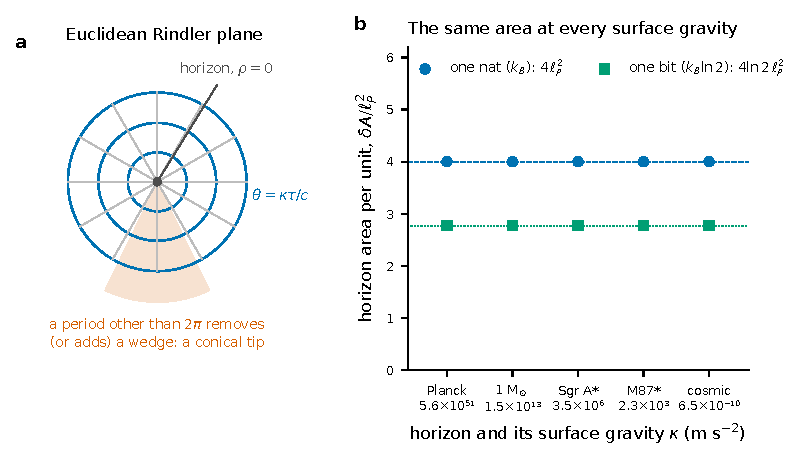
\includegraphics[width=\textwidth]{figures/part3/fig_rindler_cone.pdf}
\caption{(a) The Euclidean Rindler plane, $d\rho^2+\rho^2d\theta^2$ with $\theta=\kappa\tau/c$. With period $2\pi$ the horizon ($\rho=0$) is an ordinary point of a flat
plane; any other period removes or adds a wedge and leaves a conical tip. The period $2\pi c/\kappa$ of imaginary time is the inverse temperature,
$T=\hbar\kappa/(2\pi\kB c)$. (b) The area that one unit of entropy occupies on horizons whose surface gravities differ by 61 orders of magnitude, from the
first law $\delta(Mc^2)=(\kappa c^2/8\pi G)\,\delta A$ and the cost $\kB T$ per nat (Eq.~\eqref{eq:bk_dAmin}): $4\lP^2$ per nat and $4\ln2\,\lP^2=2.77\,\lP^2$ per bit for every
one. Planck: $\kappa=c^2/\lP$; black holes of $1$, $4.3\times10^6$ (Sgr~A$^*$) and $6.5\times10^9\,M_\odot$ (M87$^*$): $\kappa=c^4/4GM$; cosmic horizon: $\kappa=cH_0$
($H_0=67.4$, Planck 2018). \derived\ (form) \calc\ (values)}\label{fig:rindler_cone}
\end{figure}

\subsection{The $8\pi$: the Einstein equation normalization}\label{sec:bk_eightpi}
The Einstein field equations are
\begin{equation}
G_{ab}+\Lambda g_{ab}=\frac{8\pi G}{c^4}\,T_{ab}.\label{eq:bk_einstein}
\end{equation}
The coefficient $8\pi$ in Eq.~\eqref{eq:bk_einstein} is fixed by two independent geometric requirements.

\emph{(a) Gauss's law in three spatial dimensions.} In the Newtonian limit, the Einstein equations must reduce to Poisson's equation,
\begin{equation}
\nabla^2\Phi=4\pi G\rho_m.\label{eq:bk_poisson}
\end{equation}
Here $\rho_m$ is the mass density (the bare $\rho$ above is the distance from the horizon). The factor $4\pi$ is the solid angle of the unit sphere in $\mathbb R^3$,
\begin{equation}
\Omega_3=\oint d\Omega=\int_0^{2\pi}\!\!d\varphi\int_0^\pi\sin\vartheta\,d\vartheta=4\pi:\label{eq:bk_solid}
\end{equation}
the flux of $\nabla\Phi=GM\hat r/r^2$ through any sphere around a point mass is $4\pi GM$. This is a purely geometric fact about three-dimensional space.

\emph{(b) The trace factor of the Einstein tensor.} The Einstein tensor $G_{ab}=R_{ab}-\tfrac12Rg_{ab}$ differs from the Ricci tensor by the trace term
$\tfrac12Rg_{ab}$. In the weak-field limit this trace structure introduces a factor of $2$ relative to the naive identification with Poisson's equation
(Wald 1984~\cite{Wald1984}). Taking the trace of Eq.~\eqref{eq:bk_einstein} with $\Lambda=0$ gives $R=-(8\pi G/c^4)T$, so the equations can be written
$R_{ab}=(8\pi G/c^4)(T_{ab}-\tfrac12Tg_{ab})$. For static dust, $T_{ab}={\rm diag}(\rho_m c^2,0,0,0)$ and $T=-\rho_m c^2$ (signature $-+++$), and the time--time
component is
\begin{equation}
R_{00}=\frac{8\pi G}{c^4}\Big(\rho_m c^2-\tfrac12\rho_m c^2\Big)=\frac{4\pi G\rho_m}{c^2}.
\end{equation}
In the weak field $R_{00}=\nabla^2\Phi/c^2$, which is Eq.~\eqref{eq:bk_poisson}. The trace term removes half of the source, so the $4\pi$ of Gauss's law requires $8\pi$ in
front of $T_{ab}$. \derived

Combining, $8\pi=2\times4\pi$. Both factors are purely geometric. The $8\pi$ makes no reference to $\eta$, to $S\propto A$, or to the numerical value of $G$. \derived

\section{Jacobson's derivation, step by step}\label{sec:bk_jacobson}
The derivation is written out here in SI units so that the $2\pi$ and the $8\pi$ can be followed from where they enter to where they meet. Write
$\kappa_g=\kappa/c^2$ for the surface gravity in units of inverse length, which is the form in which it appears in the Killing vector.

\paragraph{Step 1: the local Rindler horizon.} Near any spacetime point $p$ the equivalence principle gives a locally flat region. Choose a small
spacelike 2-surface element $\mathcal P$ through $p$ and the past horizon of the uniformly accelerated observers just inside it: a null congruence with
tangent $k^a=dx^a/d\lambda$, affine parameter $\lambda$ (a length, zero at $\mathcal P$), and vanishing expansion and shear at $\mathcal P$. Near $p$ the
approximate boost Killing vector that generates the horizon is
\begin{equation}
\chi^a=-\kappa_g\lambda\,k^a .
\end{equation}
\emph{Assumption 1:} the vacuum fluctuations seen by the accelerated observers are thermal at the Unruh temperature Eq.~\eqref{eq:bk_unruh}, $T=\hbar\kappa/(2\pi\kB c)
=\hbar c\,\kappa_g/(2\pi\kB)$. This is where the $2\pi$ of Section~\ref{sec:bk_twopi} enters.

\paragraph{Step 2: the heat.} The heat is the boost energy that crosses the horizon,
\begin{equation}
\delta Q=\int_{\mathcal H}T_{ab}\chi^a\,d\Sigma^b=-\kappa_g\int\lambda\,T_{ab}k^ak^b\,d\lambda\,dA ,\qquad d\Sigma^b=k^b\,d\lambda\,dA .
\end{equation}
The units check: $\kappa_g$ (m$^{-1}$) $\times\lambda\,d\lambda$ (m$^2$) $\times T_{ab}k^ak^b$ (J\,m$^{-3}$) $\times dA$ (m$^2$) is an energy.

\paragraph{Step 3: the entropy.} \emph{Assumption 2:} the entropy is proportional to the horizon area, Eq.~\eqref{eq:bk_SetaA}. Then $\delta S=\kB\eta\,\delta A$
with $\delta A=\int\theta\,d\lambda\,dA$, where $\theta$ is the expansion of the generators. \derived

\paragraph{Step 4: the focusing of the generators.} The Raychaudhuri equation~\cite{Raychaudhuri1955} for the null congruence is
\begin{equation}
\frac{d\theta}{d\lambda}=-\tfrac12\theta^2-\sigma_{ab}\sigma^{ab}-R_{ab}k^ak^b .
\end{equation}
At an instantaneously stationary horizon $\theta=\sigma=0$ at $\mathcal P$, so to first order in $\lambda$ the quadratic terms drop and
$\theta=-\lambda R_{ab}k^ak^b$. Hence
\begin{equation}
\delta A=-\int\lambda\,R_{ab}k^ak^b\,d\lambda\,dA .
\end{equation}

\paragraph{Step 5: Clausius.} Setting $\delta Q=T\,\delta S$ gives
\begin{equation}
-\kappa_g\int\lambda\,T_{ab}k^ak^b\,d\lambda\,dA=\frac{\hbar c\,\kappa_g}{2\pi\kB}\,\kB\eta\Big(-\int\lambda\,R_{ab}k^ak^b\,d\lambda\,dA\Big).
\end{equation}
The surface gravity cancels. Because the relation must hold for every local horizon, through every point and for every null direction, the integrands
must agree for all null $k^a$:
\begin{equation}
T_{ab}k^ak^b=\frac{\hbar c\,\eta}{2\pi}\,R_{ab}k^ak^b\quad\text{for all null }k^a\quad\Longrightarrow\quad T_{ab}=\frac{\hbar c\,\eta}{2\pi}\,R_{ab}+f\,g_{ab},
\end{equation}
since $g_{ab}k^ak^b=0$ leaves a term proportional to the metric undetermined.

\paragraph{Step 6: conservation fixes $f$.} Matter is conserved, $\nabla^aT_{ab}=0$, and the contracted Bianchi identity gives $\nabla^aR_{ab}=\tfrac12\nabla_bR$.
Taking the divergence,
\begin{equation}
0=\frac{\hbar c\,\eta}{2\pi}\,\tfrac12\nabla_bR+\nabla_bf\quad\Longrightarrow\quad f=-\frac{\hbar c\,\eta}{2\pi}\Big(\tfrac12R-\Lambda\Big),
\end{equation}
with $\Lambda$ an integration constant. Therefore
\begin{equation}
R_{ab}-\tfrac12Rg_{ab}+\Lambda g_{ab}=\frac{2\pi}{\hbar c\,\eta}\,T_{ab}.
\end{equation}

\paragraph{Step 7: the identification.} This is the Einstein equation, Eq.~\eqref{eq:bk_einstein}, if and only if
\begin{equation}
\frac{\hbar c\,\eta}{2\pi}=\frac{c^4}{8\pi G},\qquad\text{equivalently}\qquad\frac{\hbar\eta}{2\pi}=\frac{c^3}{8\pi G},\label{eq:bk_core}
\end{equation}
which is Eq.~\eqref{eq:bk_Geta}, $G=c^3/(4\hbar\eta)$. The Einstein equation appears as an equation of state. The left-hand side carries the $2\pi$ of the Unruh
period; the right-hand side carries the $8\pi$ of the Newtonian limit. \derived

\section{The derivation of the coefficient}\label{sec:bk_derivation}
\begin{keybox}[title={Proposition (geometric determination of the entropy coefficient)}]
The numerical coefficient of the entropy--area constant $\eta$ in Jacobson's thermodynamic derivation of gravity is not a free parameter. It is
geometrically determined:
\begin{equation}
\eta=\frac{1}{4\lP^2},\qquad\frac14=\frac{2\pi}{8\pi},\label{eq:bk_eta}
\end{equation}
where $2\pi$ is the Euclidean Rindler cone angle and $8\pi$ is the Einstein equation normalization, both derivable from the causal structure of flat
spacetime without assuming $S\propto A$. The unit of area, $\lP^2=\hbar G/c^3$, carries Newton's constant. \derived
\end{keybox}

\paragraph{Derivation.} Jacobson's derivation yields the relation Eq.~\eqref{eq:bk_core}. It follows from applying $\delta Q=T\,\delta S$ to the Rindler horizon and
requiring the result to hold for all null vectors. The $2\pi$ on the left enters through the Unruh temperature (Eq.~\eqref{eq:bk_unruh}). The $8\pi$ on the right is the
Einstein normalization (Eq.~\eqref{eq:bk_einstein}). Solving for $\eta$:
\begin{equation}
\eta=\frac{c^3}{8\pi G}\cdot\frac{2\pi}{\hbar}=\frac{2\pi}{8\pi}\cdot\frac{c^3}{\hbar G}=\frac14\cdot\frac{1}{\lP^2}=\frac{1}{4\lP^2}.\label{eq:bk_etasolve}
\end{equation}
The coefficient $1/4=2\pi/8\pi$ is the ratio of the Euclidean horizon cone angle to the Einstein normalization. Both are geometric. Neither assumes
$S\propto A$. \derived

The entropy--area relation $S=\kB A/(4\lP^2)$ is therefore not a free assumption in Jacobson's framework once Newton's constant is given: it is the unique
relation consistent with the causal geometry of flat spacetime and the observed strength of gravity. Numerically, $\lP=1.61626\times10^{-35}$\,m and
$\eta=9.570\times10^{68}$\,m$^{-2}$. \calc

\paragraph{What this shows.} This is not a prediction of $\eta$ from outside Jacobson's framework, nor a claim that $\eta$ could have been derived without
Jacobson's machinery. It is a demonstration that the number in $\eta$ is geometrically fixed within that framework by the same causal geometry that
determines $T$ and $G_{ab}$. Jacobson had all the ingredients: the $2\pi$ from the Euclidean horizon geometry and the $8\pi$ from the Einstein
normalization. Their ratio $2\pi/8\pi=1/4$ fixes the coefficient without any observational input. The scale it multiplies, $c^3/\hbar G$, contains $G$,
so the matching to the observed $G$ remains the one input: given $G$, $\eta$ follows; given $\eta$, $G$ follows. The relation removes the freedom in the
number, not the need for the scale. \interp

\section{Independence of the two factors}\label{sec:bk_independence}
The derivation requires that neither factor assumes the conclusion.

The $2\pi$ from the Euclidean Rindler cone angle is a topological property of flat Minkowski spacetime near an accelerating horizon. The Euclidean
continuation of the Rindler metric produces a cone in the $(\rho,\tau)$ plane. Regularity at the tip requires the angular period to be $2\pi$ --- exactly the
period that eliminates the conical deficit. This is a statement about flat spacetime geometry, derivable without reference to black holes, entropy, or
$S\propto A$. The Bisognano--Wichmann theorem~\cite{BisognanoWichmann1976} establishes this in the full algebraic quantum field theory setting. \derived

The $8\pi$ from the Einstein normalization follows from requiring general relativity to reduce to Newtonian gravity in the weak-field, non-relativistic
limit. The factor $4\pi$ is Gauss's law in three spatial dimensions; the factor $2$ is the trace structure of the Einstein tensor. Both are geometric
properties of three-space and four-dimensional (pseudo-)Riemannian geometry respectively. Neither references entropy, Planck's constant, or $S\propto A$. \derived

\emph{Independence from each other.} The $2\pi$ is derived from quantum field theory in flat spacetime via the KMS condition. The $8\pi$ is derived from
the differential geometry of the weak-field Einstein equations. They arise from completely different physical contexts and were identified by different
historical routes --- Unruh (1976) and Einstein (1915) respectively. Their ratio appearing as the coefficient of $\eta$ is a structural consequence of
applying thermodynamics to a spacetime with both a causal horizon and a Newtonian limit. \interp

\emph{Uniqueness.} The ratio $2\pi/8\pi=1/4$ is not tunable. Both factors are fixed by geometric necessities of flat spacetime. The value $1/4$ is
selected by the geometry, not chosen to match observation. \interp

\section{Connection to known results}\label{sec:bk_known}
\subsection{The minimum encoding area: one nat per $4\lP^2$, one bit per $4\ln2\,\lP^2$}\label{sec:bk_minarea}
The same geometric ratio $8\pi/2\pi=4$ that determines $\eta$ also determines the minimum horizon area taken up by one unit of entropy. This provides an
independent confirmation that the three results --- $S\propto A$, $\eta=1/(4\lP^2)$, and the minimum encoding area --- are three expressions of the same
causal geometry. \interp

The Landauer cost of one unit of entropy, $\kB$ (one nat), at the local horizon temperature $T_H$ is
\begin{equation}
E_{\rm nat}=\kB T_H=\frac{\hbar\kappa}{2\pi c},\label{eq:bk_Enat}
\end{equation}
from the Unruh temperature (Eq.~\eqref{eq:bk_unruh}); one bit costs $E_{\rm bit}=\kB T_H\ln2$. This energy, deposited on the horizon, enlarges it by a minimum
area $\delta A_{\min}$ through the gravitational coupling. The area response of a horizon to an energy perturbation is the first law of horizon mechanics
(Bardeen, Carter \& Hawking 1973~\cite{BardeenCarterHawking1973}),
\begin{equation}
\delta(Mc^2)=\frac{\kappa c^2}{8\pi G}\,\delta A\qquad\Longrightarrow\qquad\delta A=\frac{8\pi G}{\kappa c^2}\,\delta E ,\label{eq:bk_firstlaw}
\end{equation}
where the factor $8\pi$ is the Einstein normalization (Eq.~\eqref{eq:bk_einstein}) converting energy to area perturbation, and $1/\kappa$ converts the energy at that
horizon's temperature into area. (For a Schwarzschild hole, $\kappa=c^4/4GM$ and $A=16\pi G^2M^2/c^4$ give $c^2\,dM/dA=\kappa c^2/8\pi G$ directly; for a Kerr
hole the same holds at fixed angular momentum.) Substituting Eq.~\eqref{eq:bk_Enat} into Eq.~\eqref{eq:bk_firstlaw}:
\begin{equation}
\delta A_{\min}=\frac{8\pi G}{\kappa c^2}\cdot\frac{\hbar\kappa}{2\pi c}=\frac{8\pi}{2\pi}\cdot\frac{\hbar G}{c^3}=4\lP^2 ,\label{eq:bk_dAmin}
\end{equation}
where $\lP^2=\hbar G/c^3$ was used in the last step. The surface gravity cancels: the result holds for every horizon, from the Planck-scale horizon, where
$\kappa=c^2/\lP=5.56\times10^{51}$\,m\,s$^{-2}$ is the largest surface gravity and quantum and gravitational effects are simultaneously relevant, to the cosmic
horizon with $\kappa=cH_0=6.5\times10^{-10}$\,m\,s$^{-2}$ (Fig.~\ref{fig:rindler_cone}b). \derived

The minimum horizon area taken up by one unit of entropy is $4\lP^2$. The entropy density $\eta=1/(4\lP^2)$ gives exactly one nat per $4\lP^2$:
\begin{equation}
\eta\cdot\delta A_{\min}=\frac{1}{4\lP^2}\cdot4\lP^2=1\quad\text{(one nat, $\kB$, per minimum encoding area)}.\label{eq:bk_onenat}
\end{equation}
One bit, $\kB\ln2$, occupies $4\ln2\,\lP^2=2.77\,\lP^2=7.24\times10^{-70}$\,m$^2$. \calc\ The factor of $4$ in the minimum encoding area arises from $8\pi/2\pi=4$ ---
the same ratio that determines $\eta$. This is not a numerical coincidence. It is the same geometric statement expressed twice: the ratio of the Einstein
normalization to the Euclidean horizon period determines both the entropy coefficient and the minimum encoding area, and they are consistent by
construction.

\subsection{Jacobson's machine fully specified}
Eq.~\eqref{eq:bk_core} shows that Jacobson's derivation has the structure
\begin{equation}
\underbrace{\frac{\hbar\eta}{2\pi}}_{\text{Rindler geometry}}=\underbrace{\frac{c^3}{8\pi G}}_{\text{Einstein geometry}}.\label{eq:bk_structure}
\end{equation}
Left side: the entropy--area density scaled by the Euclidean horizon period, both set by flat spacetime geometry. Right side: the gravitational coupling set
by the Newtonian limit and the trace structure of the Einstein tensor. Given $G$, the equation is satisfied if and only if $\eta=1/(4\lP^2)$; no further
observational input is required.

Jacobson's machine --- specify an entropy functional, derive a gravity theory --- then specifies its own entropy functional up to the Planck unit. The
machine is self-contained in everything but the value of $G$. \derived

\subsection{Why area scaling is geometrically necessary}
On the reading of Section~\ref{sec:bk_area}, the $S\propto A$ relation is not merely consistent with the causal geometry --- it is the unique scaling required by it.
Information from bulk decoherence events can only be permanently encoded on the causal boundary: anything inside the horizon is causally disconnected from
external observers. Bulk volume encoding would place information inaccessible to those observers. Area scaling is therefore a causal necessity
('t~Hooft 1993~\cite{tHooft1993}; Susskind 1995~\cite{Susskind1995}), and the coefficient $1/(4\lP^2)$ is the unique value consistent with the Rindler and Einstein
geometric factors derived above. \interp

\section{The remaining open problem}\label{sec:bk_open}
The results of this chapter answer three questions that Jacobson left open, at the level stated.

\emph{(A) Why does $S$ scale with $A$?} Section~\ref{sec:bk_area}: decoherence produces classical information irreversibly; permanent information must be
encoded at the causally accessible 2D boundary; volume encoding is causally forbidden. Area scaling is a necessary consequence of the causal structure.
\interp

\emph{(B) Why is the coefficient $1/4$?} Sections~\ref{sec:bk_factors}--\ref{sec:bk_derivation}: $1/4=2\pi/8\pi$, where $2\pi$ is the Euclidean Rindler cone angle and $8\pi$
is the Einstein normalization. Both are geometric facts about flat spacetime. Neither assumes $S\propto A$. \derived

\emph{(C) Why does one unit of entropy occupy $4\lP^2$?} Section~\ref{sec:bk_minarea}: the minimum horizon area taken up by one Landauer cost $\kB T_H$ is $4\lP^2$ at every
surface gravity, from the same $8\pi/2\pi=4$ ratio; one bit takes $4\ln2\,\lP^2$. The entropy coefficient and the minimum encoding area are the same
geometric fact. \derived

The remaining open question is distinct from all three. It is:
\begin{center}\emph{Why does a minimum resolvable length $\lP=\sqrt{\hbar G/c^3}$ exist at all?}\end{center}
$\lP^2=\hbar G/c^3$ is the unique area constructible from the three constants governing quantum mechanics ($\hbar$), gravity ($G$), and relativity ($c$). If a
minimum encoding area exists, it must be proportional to $\lP^2$ by dimensional necessity --- no other combination is available. But why a minimum area exists
in the first place, and why the three constants $\hbar$, $G$, $c$ combine to set it, is a question about the discrete microstructure of spacetime at the
Planck scale. This lies beyond the thermodynamic level of Jacobson's derivation and cannot be addressed from within it. It is the same question as the
value of $G$ in Section~\ref{sec:bk_derivation}: the geometry fixes the number $1/4$, and the Planck area fixes the scale. \openprob

Loop quantum gravity and string theory approach this question from different directions. The derivation here is neutral between those approaches. It
identifies $\lP^2$ as the minimum unit by dimensional necessity, and obtains all three geometric factors ($S\propto A$, the $1/4$, one nat per $4\lP^2$) from
causal spacetime structure. The single remaining gap is the quantum-gravity account of why Planck-scale discreteness exists.

\section{Discussion}\label{sec:bk_discussion}
The result is best stated precisely rather than broadly.

Jacobson's 1995 paper made two assumptions: $S\propto A$, and $\eta$ is a free parameter. Both were reasonable at the time. $S\propto A$ was motivated by the
Bekenstein--Hawking result for black holes~\cite{Bekenstein1973,Hawking1975}; $\eta$ was recovered by matching to Newton's constant. What was not recognized is how far both
assumptions follow from the causal geometry of flat spacetime.

$S\propto A$ follows, on the reading of this book, from the irreversibility of decoherence and the causal inaccessibility of the bulk: information produced
by an irreversible quantum-to-classical transition must be encoded at the 2D causal boundary because nowhere else is causally accessible to external
observers. This does not require quantum gravity; it requires only the causal structure of spacetime and the irreversibility of decoherence established
by Landauer's principle~\cite{Landauer1961} and Zurek's decoherence framework~\cite{Zurek2003}. \interp

The coefficient $1/4$ in $\eta=1/(4\lP^2)$ follows from the ratio $2\pi/8\pi$, where both factors are present in Jacobson's derivation: the $2\pi$ from the
Euclidean Rindler cone angle (Bisognano--Wichmann~\cite{BisognanoWichmann1976}), and the $8\pi$ from the Einstein normalization (Wald~\cite{Wald1984}). Jacobson had both. He did
not divide them. \derived

The minimum encoding area $\delta A_{\min}=4\lP^2$ follows from the Landauer cost of one unit of entropy at any horizon temperature, with the same $8\pi/2\pi=4$
geometric ratio. The product $\eta\,\delta A_{\min}=1$ is exact --- one nat per minimum encoding area, one bit per $4\ln2\,\lP^2$ --- and is not a separate
result but the same result stated as a consistency check. \derived

Of the two things Jacobson assumed, the number in the second is now derived and the first is given a physical reason. One thing remains open: why
Planck-scale discreteness exists at all, which is the same as asking for the value of $G$ in Planck units. That is the genuine quantum-gravity question, and
it is a much narrower and more precisely stated gap than the free coefficient it replaces. Given the Planck area, the thermodynamic level of the derivation
of $S=\kB A/(4\lP^2)$ is complete.

The thermodynamic framework of Jacobson~\cite{Jacobson1995} is the foundation of this chapter. The Unruh--Rindler geometry of Unruh~\cite{Unruh1976} and the parallel result of
Davies~\cite{Davies1975} provide the $2\pi$ factor; the Bisognano--Wichmann theorem~\cite{BisognanoWichmann1976} establishes it in the full quantum field theory setting.
Chapter~\ref{ch:blackholes} applies the coefficient to the horizon of a black hole; Chapter~\ref{ch:theory} applies the same first law to the apparent horizon of the
universe, where Cai and Kim~\cite{CaiKim2005} obtained the Friedmann equations from it.

The geometry fixes the number $1/4$, and the Planck area fixes the scale. A relativist can redo the geometry independently and check it, then take up the piece this chapter leaves open.
